\documentclass[12pt,letterpaper]{article}
\usepackage[utf8]{inputenc}
\usepackage[spanish]{babel}
\usepackage[rmargin=1.5cm,lmargin=2cm,tmargin=3.5cm,bottom=2cm]{geometry}
\usepackage{ragged2e}
\usepackage{fancyhdr}
    \pagestyle{fancy}
        \fancyhf{}
        \rhead{}
        \lhead{}

\usepackage[x11names,table]{xcolor}
\newenvironment{Figura}
  {\par\medskip\noindent\minipage{\linewidth}}
  {\endminipage\par\medskip}
\usepackage{caption}
\usepackage[rightcaption]{sidecap}

\usepackage{amsmath}
\usepackage{amssymb}
\usepackage{dsfont}
\usepackage{latexsym}
\usepackage{mathrsfs}

\usepackage{array}
\usepackage{multirow}
\usepackage{multicol}
\usepackage{colortbl}
\usepackage{tcolorbox}

\usepackage{hyperref}
\hypersetup{colorlinks=true}

\usepackage{blindtext}

\usepackage[backend=biber, citestyle=alphabetic, style=apa]{biblatex}
\bibliography{Bibliografia}

\begin{document}
%------------Pagina 1----------
\pagestyle{fancy}
        \fancyhf{}
        \lhead{}
        \rhead{\textsc{\large ARTÍCULO DE REVISIÓN}}
        \rfoot{39}
        \cfoot{\scriptsize {ISSN 0123-3122 • e-ISSN 2027-5382 • pers.bioét. • V o l . 22 • N ú m . 1 • p p . 39-55 • 2018}}
\begin{flushleft}
 \Huge \textrm{ASPECTOS BIOÉTICOS RELACIONADOS CON LA BASURA ESPACIAL Y SUS EFECTOS SOBRE LA VIDA EN LA TIERRA Y LA EXPLORACIÓN AERO ESPACIAL.}
\end{flushleft} 
\begin{flushleft}
 \large BIOETHICAL ASPECTS OF SPACE DEBRIS AND ITS EFFECTS ON LIFE 
ON EARTH AND AEROSPACE EXPLORATION

ASPECTOS BIOÉTICOS RELACIONADOS COM O DETRITO ESPACIAL

E SEUS EFEITOS SOBRE A VIDA NA TERRA E A EXPLORAÇÃO ESPACIAL
 \end{flushleft} 

\begin{flushright}
Juan Guillermo Delgado-Martínez*

Ricardo Álvarez-León**
\end{flushright}
\fbox{\parbox[b]{1.0\linewidth} {\footnotesize {\textbf {RESUMEN}}

El siglo XX fue una centuria de grandes descubrimientos científicos y desarrollos tecnológicos en todas las áreas, pero en particular 
en lo relativo a la conquista del espacio. Durante años, la bioética fue pensada en estrecha relación con la ética médica y el ámbito 
de problemas específicamente humanos, pero en los últimos tiempos su sentido se ha ido ampliando. El presente trabajo busca relacionar esta preocupación por una ciencia de la supervivencia con la existencia de la llamada basura espacial o chatarra espacial que 
orbita la Tierra, y que en un tiempo no conocido afectará pequeñas o grandes áreas de nuestro planeta. La basura espacial se ha 
convertido en una preocupación cada vez mayor, especialmente en los últimos años, puesto que las colisiones a velocidades orbitales 
pueden producir aún más basura espacial en el proceso llamado síndrome de Kessler, o cascada de ablación, lo que perjudicaría el 
funcionamiento de los satélites, afectaría las misiones espaciales o pondría en riesgo la vida de los astronautas. También es probable 
que dicha basura se precipite sobre la Tierra, con efectos no claramente evaluados sobre la población humana. Aunque el problema 
suele aparecer tanto en textos científicos como en obras de ciencia-ficción, no ha sido considerado con la seriedad exigida para un 
riesgo real y no alejado de la vida cotidiana. 

\textbf {PALABRAS CLAVE:} bioética; carrera espacial; basura espacial; riesgos; perspectivas; acciones correctivas (Fuente: DeCS).}}

\begin{flushleft}
\footnotesize {\textbf{DOI: 10.5294/PEBI.2018.22.1.4}}

{\textbf{PARA CITAR ESTE ARTÍCULO / TO REFERENCE THIS ARTICLE / PARA CITAR ESTE ARTIGO}}

Delgado-Martínez JG, Álvarez-León R. Aspectos bioéticos relacionados con la basura espacial y sus efectos sobre la vida en la Tierra y la exploración aeroespacial. pers.bioét. 2018; 22(1): 39-55. DOI: 10.5294/pebi.2018.22.1.4
\end{flushleft} 
\begin{multicols}{2}
\begin{flushleft}
\footnotesize
* orcid.org/0000-0001-9863-2206. Universidad Católica de Manizalez, Colombia. jdelgado@ucm.edu.com

** Fundación Verdes Horizontes, Colombia. 
ricardoalvarezleon@gmail.com
\end{flushleft}
\fbox{\parbox[b]{1.0\linewidth} {\footnotesize 
FECHA DE RECEPCIÓN: 2017-08-10

FECHA DE ENVÍO A PARES: 2017-08-11

FECHA DE APROBACIÓN POR PARES: 2017-11-07

FECHA DE ACEPTACIÓN: 2018-01-15}}
\end{multicols}
\newpage
%-----Pagina terminada--------------

%-----------Pagina 2----------------
\pagestyle{fancy}
        \fancyhf{}
        \rhead{}
        \lhead{\textsc{\tiny PERSONA Y BIOÉTICA • ENERO-JUNIO 201}}
        \lfoot{40}
        \cfoot{\scriptsize {ISSN 0123-3122 • e-ISSN 2027-5382 • pers.bioét. • V o l . 22 • N ú m . 1 • p p . 39-55 • 2018}}
\begin{flushleft}
\fbox{\parbox[b]{1.0\linewidth} {\footnotesize {\textbf {ABSTRACT}}

The twentieth century was a century of great scientific discoveries and technological developments in all areas, but particularly with 
regard to the conquest of space. The last stretch of the millennium also witnessed two world wars and the development of atomic
weapons with enormous destructive power, which made doubt many of the possibilities for the future of life on earth. At the end 
of his life, Albert Einstein said: “The unleashed power of the atom has changed everything except our way of thinking. So we go to 
a catastrophe unparalleled”. It is in this context of concern about the future of life on earth, Van Rensselaer Potter coined the term 
bioethics, understood as Global Bioethics, a science of survival should combine biological knowledge and human values. For years 
bioethics was thought closely related to medical ethics and scope of specifically human problems, but in recent years its meaning 
has expanded in line with the foundational approach Potter of ethics as a bridge to survival life in general. This paper seeks to relate 
this concern for a science of survival with the existence of the so-called space debris or space junk orbiting Earth and that once unknown, affect small or large areas of our planet. The waste consists of things as varied as large remnants of old rockets and satellites, 
remnants of explosions, debris or rocket components such as dust and small particles of paint. Space debris, has become a growing 
concern, especially in recent years, since collisions at orbital velocities can be highly damaging to functioning satellites, produce 
even more space debris in the process called Kessler Syndrome or waterfall ablation, but the worst would be that such wastes rush to 
land with not clearly evaluated effects on the human population. To illustrate a recent case of their impact on astronauts and equipment, it is the fact that the International Space Station had to be reinforced to mitigate the damage from this danger. Although the 
problem usually occurs both in scientific texts and works of science fiction, however it has not been considered with the seriousness 
required for a real risk and not away from everyday life.

\textbf {KEYWORDS:}  Bioethics; space race; space junk; risks; perspectives; corrective actions (Source: DeCS).}}
\fbox{\parbox[b]{1.0\linewidth} {\footnotesize {\textbf {RESUMO}}

O século XX foi um período de grandes descobertas científicas e desenvolvimentos tecnológicos em todas as áreas, mas em particular 
no tocante à conquista do espaço. Durante anos, a bioética foi pensada em estreita relação com a ética médica e com o âmbito 
de problemas especificamente humanos. Porém, nos últimos tempos, seu sentido tem sido ampliado. O presente trabalho busca 
relacionar essa preocupação por uma ciência da sobrevivência com a existência do chamado “detrito espacial” (ou “lixo espacial”) que 
orbita a Terra e que, em algum momento desconhecido, afetará pequenas ou grandes áreas do nosso planeta. Os detritos espaciais 
se converteram em uma preocupação cada vez maior, especialmente nos últimos anos, visto que as colisões em velocidades orbitais 
podem produzir ainda mais detritos espaciais no processo denominado “síndrome de Kessler”, o que prejudicaria o funcionamento 
dos satélites, afetaria as missões espaciais ou colocaria em risco a vida dos astronautas. Também é provável que tais detritos se 
precipitem sobre a Terra com efeitos não claramente avaliados sobre a população humana. Ainda que o problema costume aparecer 
tanto em textos científicos quanto em obras de ficção científica, o tema não foi considerado com a seriedade exigida para um risco 
real e próximo da vida cotidiana.

\textbf {PALAVRAS CHAVE:}ações corretivas; bioética; corrida espacial; detrito espacial; perspectivas; riscos (Fonte: DeCS, Bireme).}}

\end{flushleft}
\newpage
%-----Pagina terminada--------------

%-------Pagina 3--------------------
\pagestyle{fancy}
        \fancyhf{}
        \rhead{}
        \lhead{\textsc{\tiny ASPECTOS BIOÉTICOS RELACIONADOS CON LA BASURA ESPACIAL Y SUS EFECTOS SOBRE LA VIDA...• l JUAN GUILLERMO DELGADO-MARTÍNEZ Y OTRO}}
        \rfoot{41}
        \cfoot{\scriptsize {ISSN 0123-3122 • e-ISSN 2027-5382 • pers.bioét. • Vol.22 • Núm. 1 • pp. 39-55 • 2018}}
    
\begin{multicols}{2}
\section*{ \small {  INTRODUCCIÓN}}

\noindent El XX fue un siglo de grandes descubrimientos científicos y desarrollos tecnológicos en todas las áreas, en particular en lo relativo a la conquista del espacio. Lafotografía de Neil Armstrong en la Luna podría ser la síntesis, no solo de la carrera por la conquista espacial entre Estados Unidos y Rusia, sino de todos los avances científicos y tecnológicos de la centuria. Ocho años antes de este ícono de la tecno-ciencia, el 25 de mayo de 1961, John F. Kennedy había anunciado que Estados Unidos llevaría a un hombre a la Luna y lo traería de regreso antes de concluir la década. El presidente Kennedy fue asesinado en 1963 y no pudo ver su sueño cumplido, aunque sí lo hicieron, en cambio, gracias a la enorme difusión de la televisión, millones de personas en todo el mundo. Junto con la ilusión por conquistar el espacio y llegar a “donde nunca nadie ha llegado antes”, como decía el lema de la tripulación de la nave futurista USS Enterprise (NCC-1701), el último tramo del milenio presenció dos grandes guerras mundiales y el desarrollo de armas atómicas con un enorme poder destructivo, lo que hizo dudar a muchos de las posibilidades de futuro de la vida sobre la Tierra. Al final de su existencia, Albert Einstein dijo: “La fuerza desencadenada del átomo lo ha transformado todo, menos nuestra forma de pensar.Por eso vamos hacia una catástrofe sin igual” (1). Es precisamente en este contexto de ilusión y preocupación sobre el futuro de la vida sobre la Tierra, que V. R. Potter acuña el término Bioética, entendida como Global Bioethics, una ciencia de la supervivencia que debería aunar conocimientos biológicos y valores humanos.
Durante años, la bioética fue pensada en estrecha relación con la ética médica y con el ámbito de problemas específicamente humanos, pero en los últimos años su sentido se ha ido ampliando, en la línea del planteamiento fundacional de Potter, a una ética como puente hacia la supervivencia de la vida en general. El presente trabajo busca relacionar esta preocupación por una ciencia de la supervivencia con la existencia de la llamada basura espacial o chatarra espacial que orbita nuestro planeta y que, eventualmente, afectaría a la población humana sobre la Tierra. Entre las diferentes áreas de la bioética se suele distinguir una bioética general, encargada de ofrecer una fundamentación histórica, antropológica y epistemológica; la bioética especial se refiere a áreas o problemas específicos relacionados, por ejemplo, con el inicio y el final de la vida, con la sexualidad humana, entre otras, y busca aplicar los principios de la bioética general a dichos problemas.


\section*{\small{EL RETORNO A LA BIOÉTICA DE POTTER:
GLOBAL BIOETHICS}} 
\noindent A pesar del éxito y la enorme difusión del término bioética (publicaciones, institutos de investigación, congresos, grados y posgrados, declaraciones, entre otros), muchas personas con formación universitaria aún no poseen una idea de a qué se dedica esta joven disciplina. Incluso para los ya iniciados es probable que los temas que vengan primero a la mente sean los del aborto, la eutanasia, la fecundación in vitro, entre otros, por tratarse de asuntos amplia y largamente discutidos en los medios de comunicación. La bioética, así entendida, aparece como el nuevo nombre o derivación de la tradicional ética médica, que interesaría sobre todo al personal de la salud y a quienes se preocupan por los problemas éticos asociados a la clínica y la salud pública. 
\end{multicols}
\newpage
%-----Pagina terminada--------------

%------------Pagina 4----------
\pagestyle{fancy}
        \fancyhf{}
         \lfoot{42}
        \lhead{\textsc{\tiny PERSONA Y BIOÉTICA • ENERO-JUNIO 201}}
        \cfoot{\scriptsize {ISSN 0123-3122 • e-ISSN 2027-5382 • pers.bioét. • V o l . 22 • N ú m . 1 • p p . 39-55 • 2018}}
\begin{multicols}{2}
\\
\noindent Pero al inicio no era así. Cuando V. R. Potter acuñó el término bioética a comienzos de la década de 19701, la entendió fundamentalmente como una bioética global \textit{(Global Bioethics)}, un puente hacia el futuro que permitiría la supervivencia, no solo de la vida humana, sino de la vida en general. Como señala Elena Postigo,Solana: 
\\

  \begin {itemize}
    \item[\textcolor{white}{x}]… la teoría original de la bioética era la intuición que señalaba que la supervivencia de gran 
alcance de la especie humana, en una civilización decente y sustentable, requería del desarrollo y del mantenimiento de un sistema ético. Tal sistema es la Bioética Global, basada en intuiciones y razonamientos sustentados en el conocimiento empírico proveniente de todas las ciencias, pero en especial del conocimiento biológico. En esta observación utilizo la palabra empírico en el sentido usual: el conocimiento empírico es el conocimiento basado en observaciones o experimentos que son independientemente verificables. En la actualidad, este sistema ético 
  \end{itemize} 
\\

\noindent \rule{50mm}{0.1mm}

\noindent {\footnotesize Hoy se sabe que no fue Potter, sino el pastor alemán 
protestante Fritz Jahr quien usara por primera vez el término 
Bioética en 1926 en un artículo titulado “La ciencia de la vida 
y la enseñanza de la moral. Viejos descubrimientos bajo una 
nueva luz”. Posteriormente, en un artículo aparecido en 1927, 
titulado “Bio-ética: un análisis de las relaciones éticas de los 
seres humanos con los animales y las plantas” publicado como 
editorial en la revista alemana Kosmos.}
\\
\\
\\
\\
\\
\begin {itemize}
    \item[\textcolor{white}{x}]propuesto sigue siendo el núcleo de la bioética puente con su extensión a la bioética global, en la que la función de puente ha exigido la fusión 
de la ética médica y de la ética medioambiental en una escala de nivel mundial para preservar la supervivencia humana.
  \end{itemize} 
\\
\\
Sin embargo, el desarrollo inmediatamente posterior de la bioética se enfocó en el ámbito clínico y de la salud humana como lo muestran los hitos que se suelen citar como constitutivos de la historia de la bioética. Por ejemplo, los experimentos de los médicos nazis con prisioneros en los campos de concentración, sin ningún tipo de consentimiento informado (aunque anteriores en el tiempo respecto al uso del término bioética, estos desmanes de los galenos en los campos de concentración serían juzgados en Nuremberg, y permitirían la aparición del llamado Código de Nuremberg que regula la experimentación médica en seres humanos. Este código, con su especial énfasis en el consentimiento informado, se suele considerar un acontecimiento fundamental en el nacimiento de la bioética), el experimento Tuskegee con población afrodescendiente afectada por la sífilis, así 
como los realizados en elJewish Chronic Disease Hospital de Brooklyn con ancianos a quienes se les inyectaron células cancerígenas y el Willobrock State Hospital de Nueva York, a niños con deficiencia mental a quienes les inocularon el virus de la hepatitis. Por otra parte, el famoso modelo de una bioética principialista, aún vigente en muchos lugares, se inspiró en buena parte en el libro Principios de ética biomédica de Tom Beauchamp y James Childress (4) que, como su nombre lo indica, fue pensado para el ámbito biomédico. Las inquietudes y polémicas mediáticas sobre el acceso a los primeros centros de diálisis externa, así como el nacimiento en 1978 de Luisa Brown, la primera bebé probeta, parecían
\end{multicols}
\newpage
%-----Pagina terminada-----

%---------Pagina 5---------
\pagestyle{fancy}
        \fancyhf{}
        \rhead{}
        \lhead{\textsc{\tiny ASPECTOS BIOÉTICOS RELACIONADOS CON LA BASURA ESPACIAL Y SUS EFECTOS SOBRE LA VIDA...• l JUAN GUILLERMO DELGADO-MARTÍNEZ Y OTRO}}
        \rfoot{43}
        \cfoot{\scriptsize {ISSN 0123-3122 • e-ISSN 2027-5382 • pers.bioét. • Vol.22 • Núm. 1 • pp. 39-55 • 2018}}
  \begin{center}
  \textrm{CADA VEZ PARECE MÁS CLARO QUE LA VIDA Y LA SALUD DE LA HUMANIDAD NO PUEDEN
SER ENTENDIDAS DE FORMA AISLADA, YA QUE EL SER HUMANO HACE PARTE DE UN COMPLEJO
ECOSISTEMA DONDE LA ACCIÓN LIBRE DEL HOMBRE NO SOLO PUEDE AFECTAR LA SUSTENTABILIDAD
DE OTRAS FORMAS DE VIDA SOBRE LA TIERRA, SINO TAMBIÉN LA MISMA VIDA HUMANA.}
\\
  \end{center}
  
\begin{multicols}{2}
\\
\noindent encarrilar definitivamente a la joven disciplina en los rieles de la tradicional ética médica y clínica.
\\
\\
Pero en las últimas dos décadas, y cada vez con más 
fuerza, se percibe un renovado interés de los bioeticistas allende los problemas ya referidos de la salud y la vida humana. Los manuales de bioética no hablan ya solo de aborto, eutanasia, trasplantes y sexualidad humana, sino que se ven obligados a incluir largos capítulos sobre medio ambiente, biotecnologías animales y vegetales, organismos genéticamente modificados, entre otros. El cambio climático y la contaminación asociada a hábitos 
consumistas de muchas sociedades, la escasez de recursos naturales como el agua, y la pérdida de biodiversidad en plantas y animales evidencia que a la intervención utilitaria y pertinaz del hombre sobre la naturaleza se debe sumar una nueva conciencia, respetuosa de los ritmos y las posibilidades de la misma. La acción del hombre en el mundo a través de la técnica no es neutra, sino que afecta a los ecosistemas, y el equilibrio de estos repercute a su vez en la salud y el bienestar de las sociedades humanas. Un ejemplo de ello es Pekín, capital de China y primer emisor de CO2 en el mundo, que se ve obligada a cerrar sus fábricas, con gran afectación económica, cuando se presenta la temida alerta roja que avisa de los altos niveles de partículas contaminantes en el aire. Esta alerta se activa cuando las partículas contaminantes en el aire superan los 452 μgr/m3
/24 h. La Organización Mundial de la Salud (OMS), por su parte, advierte que el nivel máximo recomendado es de 25 μgr/m3
/24 h (5). No solo se afectan, por supuesto, la industria y la economía. El impacto más grave ocurre sobre la población. La contaminación atmosférica es la causante, anualmente, de la muerte de cientos de miles de personas en China y de millones en todo el mundo (6).
\\

\noindent A la contaminación del aire por parte de la industria se añade su relación con el cambio climático y la consecuente afectación de las comunidades más pobres y vulnerables que no cuentan con los medios suficientes para adaptarse o hacer frente a eventuales catástrofes (7). Se pueden mencionar muchos más ejemplos referentes al acceso y calidad de agua, el abuso de los recursos naturales, la pérdida de amplias zonas de bosques, el agotamiento de reservas ictícolas, entre tantas otras, que ponen en peligro la biodiversidad del planeta y la supervivencia humana, según el original planteamiento de Potter.
\\

\noindent Cada vez parece más claro que la vida y la salud de la humanidad no pueden ser entendidas de forma aislada, ya que el ser humano hace parte de un complejo ecosistema donde la acción libre del hombre no solo puede afectar la sustentabilidad de otras formas de vida sobre la Tierra, sino también la misma vida humana.
\end{multicols}
\newpage
%-----Pagina terminada-----

%---------Pagina 6--------
\pagestyle{fancy}
        \fancyhf{}
        \rhead{}
         \lhead{\textsc{\tiny PERSONA Y BIOÉTICA • ENERO-JUNIO 201}}
        \lfoot{44}
        \cfoot{\scriptsize {ISSN 0123-3122 • e-ISSN 2027-5382 • pers.bioét. • Vol.22 • Núm. 1 • pp. 39-55 • 2018}}
  
\begin{multicols}{2}
En ese sentido, ecología y bioética no constituirían dos disciplinas diferentes con algunos puntos de contacto, sino que más bien una incluiría la otra (7).

\section*{\noindent \small {LOS RETOS DE LA BIOÉTICA EN LA CARRERA ESPACIAL}}

\noindent La película de animación Wall-E, de 2008, del famoso director Andrew Stanton, imaginaba el futuro del planeta Tierra, en el año 2700, lleno de escombros. Los seres humanos habían emprendido un crucero galáctico escapando de unos altísimos niveles de toxicidad, mientras que un batallón de robots, entre ellos el protagonista Wall-E, se encargaban de la limpieza. La especie humana,en busca de su supervivencia, habría debido escapar de la contaminación que ella misma habría producido.En una de las escenas, poco antes de que A. Stanton nos muestre qué ha sido de la raza humana, vemos despegar de la Tierra una nave llevando a bordo a Eva, la elegante robot que busca indicios de vida en la superficie terrestre, y también a Wall-E, el laborioso e inquieto recolector de basura. La nave debe hacerse paso entre cientos de satélites abandonados, escombros y residuos que cubren la tierra como una nube metálica, antes de emprender su viaje hacia el Axioma, nave en la que se encontraría la humanidad. Es una simple escena de una película animada, pero no está tan lejos de la realidad 
como podría pensarse (8).
\\

\noindent En 1955, tanto Estados Unidos como la URSS anunciaron públicamente su intención de lanzar en los años siguientes satélites artificiales al espacio, como contribución al Año Geofísico Internacional (1957-1958).La carrera espacial fue una competencia entre Estados Unidos y la URSS, que se extendió aproximadamente desde 1957 hasta 1975. Supuso el esfuerzo paralelo entre ambos países de explorar el espacio exterior con satélites artificiales, de enviar humanos al espacio y de posar a un ser humano en la Luna. Aunque sus raíces están en las primeras tecnologías de cohetes y en las tensiones internacionales que siguieron a la Segunda Guerra Mundial, la carrera espacial comenzó de hecho tras el lanzamiento soviético del Sputnik 1 el 4 de octubre de 1957. El término carrera se originó como analogía de la competencia armamentista. La carrera espacial se convirtió en una parte esencial de la rivalidad cultural y tecnológica entre la URSS y Estados Unidos durante la Guerra Fría. La tecnología espacial llegó a ser una arena particularmente importante en este conflicto, tanto por sus potenciales aplicaciones militares como por sus efectos psicológico sobre la moral de la población (9).
\\

\noindent No obstante, con la carrera espacial iniciada el siglo pasado, no solo el hombre alcanzó el espacio, lo hizo también su basura. Con la expresión space debris (o también orbital debris) nos referimos a elementos de origen humano, ya no útiles, provenientes de explosiones, colisiones o desprendimientos de cohetes o satélites viejos. En primer lugar habría que destacar lo novedoso de este tipo de basura, no era posible hablar de ella antes del siglo XX ya que el ser humano no había logrado enviar objetos fuera de la atmósfera terrestre. Es posible, entonces, datar el inicio de esta basura en la década de 1950, más exactamente en octubre de 1957, corazón de la Guerra Fría, cuando el primer satélite, el Sputnik 1, fuera enviado al espacio. Lo siguieron el Sputnik 2 y el estadounidense Explorer 1. La conquista por el espacio llegó a ser el símbolo de la competencia por el reconocimiento de la superioridad en todos los campos. Ser los primeros en enviar un objeto, un animal o a un ser
humano al espacio no era una mera opción. Era la tarea fundamental. Aún hoy, objetos enviados 

\end{multicols}
\newpage
%-----Pagina terminada-----

%---------Pagina 7--------
\pagestyle{fancy}
        \fancyhf{}
        \rhead{}
         \lhead{\textsc{\tiny ASPECTOS BIOÉTICOS RELACIONADOS CON LA BASURA ESPACIAL Y SUS EFECTOS SOBRE LA VIDA...• l JUAN GUILLERMO DELGADO-MARTÍNEZ Y OTRO}}
        \rfoot{45}
        \cfoot{\scriptsize {ISSN 0123-3122 • e-ISSN 2027-5382 • pers.bioét. • Vol.22 • Núm. 1 • pp. 39-55 • 2018}}
  
\begin{multicols}{2}
\noindent hace más de cincuenta años hacen su reentrada en la 
atmósfera terrestre: “La nave más antigua en hacer su reentrada el año pasado [2015] fue el satélite ruso de telecomunicaciones Molniya 1/42, lanzado en 1978; y el escombro de origen más antiguo que hizo su reentrada también en 2015 fue un fragmento asociado al Vanguard 3, lanzado por Estados Unidos en 1959” señala Eduardo García-Llama (10), quien trabajó en el Centro Europeo de Investigación y Tecnología Espacial de la Agencia Espacial Europea en Holanda. Con la multiplicación de satélites e investigaciones aeroespaciales esta basura ha ido en aumento y se ha convertido en una preocupación a causa de los perjuicios que podría generar en el funcionamiento de satélites, naves y misiones espaciales, además del peligro para la vida humana de los astronautas implicados. Por si fuera poco, a ello se sumaría el llamado síndrome de Kessler (11), también conocido como cascada de ablación. Este predice que la cantidad de basura espacial presente en la órbita baja terrestre, la que se encuentra entre los 200 y 2.000 km sobre la superficie de la Tierra, sería tan alta que ocasionaría una gran cantidad de colisiones, una especie de efecto dominó, multiplicando a su vez el número de escombros y dificultando aún más el uso de la órbita baja de la Tierra hasta hacerla inutilizable.
\\

\noindent Las misiones espaciales lanzadas a la órbita de la Tierra han sido tripuladas por hombres y mujeres ampliamente entrenados para desempeñarse en el ámbito de ingravidez durante largos periodos. Las misiones no tripuladas por seres humanos, excepcionalmente han incluido animales (perros y simios), dentro de los satélites y las sondas. Han sido puestos en órbita diferentes satélites 
por Alemania en 1944, la URSS desde 1957 (Sputnik 2 
+ la perra Laika), USA desde 1958 (Programa Mercurio, 
Cohete Little Joe 2 + el macaco Sam), Francia desde
\\

\begin{center}
AÚN HOY, OBJETOS ENVIADOS HACE MÁS
DE CINCUENTA AÑOS HACEN SU REENTRADA
EN LA ATMÓSFERA TERRESTRE: “LA NAVE
MÁS ANTIGUA EN HACER SU REENTRADA
EL AÑO PASADO [2015] FUE EL SATÉLITE
RUSO DE TELECOMUNICACIONES MOLNIYA
1/42, LANZADO EN 1978; Y EL ESCOMBRO
DE ORIGEN MÁS ANTIGUO QUE HIZO SU
REENTRADA TAMBIÉN EN 2015 FUE UN
FRAGMENTO ASOCIADO AL VANGUARD 3, 
LANZADO POR ESTADOS UNIDOS EN 1959”.
\end{center}
\\

\noindent 1965 (Vesta + macaco Martine en 1967), Argentina desde 1969 (Canopus II + mono caí Juan), Japón desde 1970 (Ohsumi), UK desde 1971 (Prospero X-3), Europa desde 1979 (Spot), India desde 1981 (Rhohini), Rusia desde 1982 (Cosmos 1413, Cosmos 1414, Cosmos 1415), Israel desde 1988 (Ofeq), Canadá desde 1998 (Zaryá), China desde 2001 (Shenzhou 2), Irán desde 2008 (Omid), Corea del Norte desde 2012 (Kwangmyŏngsŏng-3), y vuelos privados desde 1997 (Celestis 01). Estas misiones han tenido multitud de éxitos, de fracasos, de objetivos cumplidos parcialmente, que han marcado verdaderos hitos en la historia aeroespacial (12). E. García-Llama calcula que habría cerca de 17.000 objetos artificiales con un tamaño igual o mayor a los diez centímetros en órbita alrededor de la Tierra (13). La mayoría de estos fragmentos provienen de explosiones y colisiones. Es probable que la mayor explosión fuera la 
\end{multicols}
\newpage
%-----Pagina terminada----

%---------Pagina 8--------
\pagestyle{fancy}
        \fancyhf{}
        \rhead{}
        \lhead{\textsc{\tiny PERSONA Y BIOÉTICA • ENERO-JUNIO 201}}
        \lfoot{46}
        \cfoot{\scriptsize {ISSN 0123-3122 • e-ISSN 2027-5382 • pers.bioét. • Vol.22 • Núm. 1 • pp. 39-55 • 2018}}
  
\begin{multicols}{2}
\noindent ocasionada intencionalmente en enero de 2007 por un misil chino al satélite –también chino– Fengyun 1C en el marco de una demostración militar, y que produjo cerca de 4.000 escombros (bastó uno solo de estos restos para inutilizar al pequeño satélite ruso Blits al golpearlo en enero de 2013). La mayor colisión accidental ocurrió dos años después, en febrero de 2009, entre dos satélites, el estadounidense Iridium 33 y el ruso Kosmos 2251, que causó cerca de 2.000 fragmentos más. Solo estos residuos orbitales conjuntos de la maniobra militar china y del accidente entre los dos satélites equivalen a un 35\% de la basura espacial mayor a 10 cm. El otro 65\% restante serían, en su mayoría, satélites, etapas de cohetes sin o con poco combustible que estuvieron destinadas a lanzar satélites, o elementos eyectados por vehículos o satélites durante su funcionamiento normal.
\\

\noindent La historia reciente y los cálculos probabilísticos afirman que esta basura podría poner en un serio peligro el éxito de misiones espaciales presentes y futuras. Pero estos riesgos, entendidos como “disvalores posibles”(14), no solo amenazan una pluralidad de valores como los científicos, tecnológicos, económicos y políticos ligados a la exploración y conquista espacial (15); también ponen en juego la seguridad y la salud de los astronautas involucrados en estas misiones, así como la de individuos y poblaciones humanas que eventualmente se verían afectadas por las precipitaciones de algunos de estos materiales.
\\

\section*{\noindent \small {CAUSAS DE LA CONTAMINACIÓN ESPACIAL}}
\\

\noindent Los satélites inservibles, las etapas y los equipos astronáuticos, o las plataformas
de investigación, se pasean por nuestra órbita planetaria de forma arbitraria y sin ningún tipo de control. Cuando entran por azar –o debido al desgaste y la corrosión– en el ámbito terrestre hacen su aparición según las normas físicas del rozamiento espacial.
\begin{enumerate}
    \item Las explosiones de las etapas superiores de los cohetes de lanzamiento suponen la contribución más importante al problema de la basura espacial. Cerca de 100 toneladas de fragmentos generados durante aproximadamente 200 explosiones todavía están en órbita. La basura espacial se concentra más en la órbita baja de la tierra, aunque algo se extiende hacia más allá de la órbita geoestacionaria. A finales de 2003 había unos 10.000 objetos catalogados. No obstante, se estima en más de 50.000 el número de objetos mayores de un centímetro. Según la revista Nature, Estados Unidos tiene registrados en la actualidad más de 9.000 objetos artificiales, con un peso total que supera las cinco toneladas. La mayor parte de estos aparatos están en ruina y constituyen un gran riesgo para las misiones espaciales. En la actualidad, según el informe de la Oficina del Programa de la NASA de Restos Orbitales se estima que existen 16.602 escombros de satélites y cohetes orbitando nuestro planeta.
    \item En enero 11 de 2007, los chinos lanzaron un misil balístico de rango medio desde su centro espacial de Xiang Space. Ascendió como lo que era, un cohete, y a una órbita de baja altitud –865 km– impactó contra un viejo satélite meteorológico, el Feng Yun 1C, que en una décima de segundo quedó convertido en 2.000 fragmentos de entre 5 y 10 cm de lado, 35.000 de alrededor de 1 cm y cerca de un millón de pedacitos de más o menos 1 mm. Esa era la misión encomendada al misil antisatélites. En esa décima de segundo, el volumen de desechos espaciales que orbitan en torno de la Tierra aumentó en cerca de un 15\%.
\end{enumerate}
\end{multicols}
\newpage
%-----Pagina terminada----

%---------Pagina 9--------
\pagestyle{fancy}
        \fancyhf{}
        \rhead{}
        \lhead{\textsc{\tiny ASPECTOS BIOÉTICOS RELACIONADOS CON LA BASURA ESPACIAL Y SUS EFECTOS SOBRE LA VIDA...• l JUAN GUILLERMO DELGADO-MARTÍNEZ Y OTRO}}
        \rfoot{47}
        \cfoot{\scriptsize {ISSN 0123-3122 • e-ISSN 2027-5382 • pers.bioét. • Vol.22 • Núm. 1 • pp. 39-55 • 2018}}
  
\begin{multicols}{2}
\begin{itemize}
    \item[3]Estados Unidos y la URSS, que dominaban esa tecnología balística desde hacía tres décadas, dejaron de ensayar sus misiles en la década de 1980 precisamente para no saturar el inmenso basurero espacial en torno al planeta. El 19 de febrero de 2007, una etapa del tipo Briz-M del cohete ruso Protón lanzado un año antes en una misión fallida, y que había quedado en órbita con todo su combustible, explotó por la elevada temperatura derivada del rozamiento con la atmósfera. Un millar de grandes fragmentos, de entre 1 y 10 cm, quedó dando vueltas en torno a la Tierra.
    \item [4] La basura espacial se origina principalmente en explosiones de satélites o partes de cohetes. El desprendimiento de las distintas etapas de un cohete, como en el caso del histórico cohete Saturno V, que llevó al hombre a la Luna, también ha sido una fuente común de desperdicio. Muchas veces las baterías de los satélites estallan accidentalmente; en otros casos, satélites fuera de órbita han sido destruidos intencionalmente para evitar su entrada a la Tierra.Existe una lista de 115 misiones que han terminado en la destrucción o fragmentación de satélites, naves o cohetes, lista necesariamente incompleta por la restringida información acerca de satélites espías. Como sea, el primer registro “oficial” de la generación de basura espacial corresponde al desprendimiento de una etapa del cohete Ablestar que puso en órbita al satélite Transit 4A, el 29 de junio de 1961. Tres años después se dio la primera destrucción intencional de un satélite, el Kosmos 50, al no ser recobrado acorde a lo planeado por los soviéticos que lo pusieron en órbita. En muchas ocasiones, tanto soviéticos como estadounidenses hicieron pruebas haciendo explotar deliberadamente satélites en órbita. Eventualmente todas estas explosiones dieron lugar al problema actual de los desechos espaciales (16). 
    \item [5]Todo comenzó con el Sputnik en 1957, es decir, con el lanzamiento de este satélite comenzó a generarse la basura espacial. Desde entonces se han puesto en órbita más de 5.000 satélites, los cuales, conforme van cumpliendo su tiempo de vida útil, son abandonados. Actualmente existen tres órbitas que almacenan basura: la órbita baja (LEO), la órbita cementerio (17) y la órbita geoestacionaria. La geoestacionaria es la más preocupante, pues es donde se encuentran situados los satélites, aproximadamente a 35.786 km de la Tierra (18). Se estima que hay en ella unos 3.000 fragmentos de diferentes tamaños (de entre 15 cm y 1 m) y donde se pueden hallar objetos de lo más diverso, desde una simple botella, hasta material de reparación y montaje, pasando por restos de satélites dañados o accidentados. El cohete Pegasus, por ejemplo, enviado al espacio en 1994, explotó dos años después y generó varios cientos de miles de fragmentos. Incluso los más milimétricos son sumamente peligrosos. Un diminuto fragmento de pintura que impacte el traje de un astronauta que realice un paseo espacial le causaría la muerte en el acto, ya que la mayoría de ellos viajan a varias docenas de miles de kilómetros por hora. Para un ejemplo aún más elocuente, en 1965 el astronauta Edward White perdió un guante de unos 30 cm en el espacio, el cual se desintegró en la atmósfera un mes después, pero mientras tanto estuvo viajando a 28.000 km/h, una velocidad tal, que si una nave interceptase el guante en su camino quedaría destruida. En 1979, la National Aeronautics and Space Administration de Estados Unidos (NASA) registró 
\end{itemize}
\end{multicols}
\newpage
%-----Pagina terminada----

%---------Pagina 10--------
\pagestyle{fancy}
        \fancyhf{}
        \rhead{}
        \lhead{\textsc{\tiny PERSONA Y BIOÉTICA • ENERO-JUNIO 201}}
        \lfoot{48}
        \cfoot{\scriptsize {ISSN 0123-3122 • e-ISSN 2027-5382 • pers.bioét. • Vol.22 • Núm. 1 • pp. 39-55 • 2018}}
\begin{multicols}{2}
\begin {itemize}
    \item[\textcolor{white}{x}]que ya habían sido lanzados al espacio 11.366 objetos espaciales de los cuales 4.633 objetos, y luego unos 6.733, ya habían entrado en la atmósfera de la Tierra. Nueve años más tarde, en 1989, la Comisión Nor-teamericana de Defensa Aeroespacial (Norad), que tiene  la  capacidad  de  reunir  objetos  en  el  espacio  del tamaño de 10 cm de diámetro, a una distancia de 500 km, registró que habían sido lanzados un total de  19.037  objetos  al  espacio,  de  los  cuales  unos  12.000 habían ingresado en la atmósfera terrestre. De esos objetos espaciales, que si bien constituyen un testimonio del progreso logrado en la exploración y explotación del espacio ultraterrestre, un 95\% hoy en día no funcionan, no se controlan y componen lo que se llama basura o desechos espaciales. En ese sentido, el Comité Internacional de Coordinación de Escombros Espaciales (Inter-Agency Space Debris Coordination Committee), que agrupa trece agen-cias  espaciales  de  diferentes  países  y  colectivos  de  países,  se  empeña  en  “avanzar  en  el  conocimiento  de la basura espacial y en desarrollar estrategias de gestión ambiental para preservar el espacio cercano a la Tierra para las futuras generaciones” (19) 
  \end{itemize} 
\section*{\noindent \small {LA CONTAMINACION Y LA BASURA ESPACIAL}}
\\
\noindent Uno  de  los  resultados  más  indeseables  de  la  carrera  espacial inicialmente entre Estados Unidos y la Unión Soviética,  y  luego  de  otras  naciones  que  poco  a  poco  han ido entrando en esta competencia tecnológica, es la llamada basura espacial, chatarra espacial o space debris, es decir cualquier objeto artificial sin utilidad que orbita la Tierra. Se compone de cosas tan variadas como grandes restos de cohetes y satélites viejos, restos de explosio-nes, o restos de componentes de cohetes como polvo y pequeñas partículas de pintura. En resumen, la basura aeroespacial es otro invento del hombre que también nos acorrala día a día y afecta nuestra ecología humana (20).La basura espacial se ha convertido en una preocupación cada vez mayor en estos últimos años, puesto que las colisiones a velocidades orbitales pueden ser altamente perjudiciales para el funcionamiento de los satélites y pueden también producir aún más basura espacial en un proceso llamado Síndrome de Kessler. La primera maniobra oficial de una nave tripulada para evitar una colisión fue la del Discovery STS-48 en septiembre de 1991. Durante 7 segundos se realizó un encendido del sistema de control para evitar un posible encuentro con restos del satélite Kosmos 955. Los expertos reconocen que hacer frente a este problema es complicado y costoso, por lo que sería necesario que los investigadores idearan nuevos métodos para solucionar esta clase de problemas.
\\

\noindent La  Estación  Espacial  Internacional  o  International  Space Station (ISS), que comenzó su construcción en órbita desde 1998, tuvo que ser blindada para atenuar los daños debido a este peligro. El proyecto funciona como una estación espacial permanentemente tripulada, en la que rotan equipos de astronautas e investigadores de las cinco agencias del espacio participantes –la NASA, la Agencia  Espacial  Federal  Rusa  (FKA),  la  Agencia  Japonesa  de  Exploración  Espacial  (JAXA),  la  Agencia  Espacial Canadiense (CSA) y la Agencia Espacial Eu-ropea (ESA)– está considerada como uno de los logros más  grandes  de  la  ingeniería.  La  basura  espacial  ha  puesto  en  peligro  a  los  tripulantes  de  la  ISS.  Aunque  los desperdicios pasaron a 250 m, los seis astronautas que permanecían a bordo se vieron obligados a reali-zar maniobras de evacuación y a refugiarse en las dos naves Soyuz acopladas a la estación.
\end{multicols}
\newpage
%-----Pagina terminada----

%---------Pagina 11-------
\pagestyle{fancy}
        \fancyhf{}
        \rhead{}
        \lhead{\textsc{\tiny ASPECTOS BIOÉTICOS RELACIONADOS CON LA BASURA ESPACIAL Y SUS EFECTOS SOBRE LA VIDA...• l JUAN GUILLERMO DELGADO-MARTÍNEZ Y OTRO}}
        \rfoot{49}
        \cfoot{\scriptsize {ISSN 0123-3122 • e-ISSN 2027-5382 • pers.bioét. • Vol.22 • Núm. 1 • pp. 39-55 • 2018}}
        \begin{multicols}{2}
\section*{\noindent \small {RIESGOS PARA LAS MISIONES ESPACIALES}}

\noindent La probabilidad actual de una colisión causada por la presencia  de  la  basura  espacial  es  muy  baja.Sin  embargo, no parece prudente minusvalorar este riesgo, en especial  cuando,  como  señalan  Jean-Michel  Courty  y  Édouard Kierlik, “algunas órbitas ya comienzan a estar tan atiborradas que, antes o después, el riesgo de choque acabará siendo inaceptable” (21).
\\

\noindent En mayo de 2016, el diario El País hacía eco en su edición digital del inicio de operaciones de un observatorio de asteroides, satélites y basura espacial en la montaña de Niefla, Puertollano (Ciudad Real) en Castilla-La Mancha (“Un observatorio de basura espacial comienza a operar en Puertollano”), dirigido por el astrónomo Jaime Nomen. Gian María Pinna, de la Agencia Europea del Espacio (ESA), responsable de proyecto europeo de vigilancia espacial  para  España,  afirmaba  en  esta  nota  que:  “la  basura espacial es un problema muy real: necesitamos saber dónde está la basura espacial para poder mover los  satélites  operativos  y  evitar  colisiones”,  y  añadía:  “con todos nuestros satélites en órbita [...] tenemos que realizar maniobras con un par de ellos cada semana para evitar colisiones con restos de basura” (22).
\\

\noindent También en mayo de 2016 resultó ser una gran noticia el que un minúsculo fragmento de basura espacial gol-peara una ventana de la ISS. Como era un objeto muy pequeño  no  supuso  ningún  riesgo  para  la  misión  de  la Estación ni para su tripulación. Vale la pena anotar que estos fragmentos que giran alrededor de la Tierra alcanzan velocidades cercanas a los 7 u 8 km/s. Si a ello se suma la consideración de la velocidad relativa, dado que es probable que el objeto impactado presente tam-bién una alta velocidad, esto explica cómo elementos tan pequeños sean tan potencialmente destructivos. ¿Qué hubiese  ocurrido  si  el  fragmento  que  golpeó  a  la  ISS  tuviera un tamaño superior a los 10 cm? Se piensa que un residuo de basura del tamaño de un grano de arroz podría  desestabilizar  o  hacer  inutilizable  un  satélite,  mientras que el impacto de un fragmento de un tamaño igual o mayor a 10 cm ocasionaría daños irreparables en el artefacto impactado o incluso su destrucción total.
\\

\noindent Resulta significativo que la ISS haya tenido que realizar durante los años 2014 y 2015 nueve maniobras evasivas frente a una probable colisión, el mismo número de ma-niobras que, como lo muestra la figura 1, debió realizar durante los diez años precedentes, los que van del 2004 al 2013. Cada una de estas maniobras tarda cerca de 30 horas para ser correctamente planeada y ejecutada. No solo la ISS debió realizar maniobras evasivas: “La NASA ejecutó hasta 26 maniobras evasivas en algunos de sus satélites  durante  2015,  5  de  ellas  para  evitar  posibles  impactos con fragmentos del satélite chino Fengyun-1C y 8 para evitarlos con los procedentes de la colisión entre el  Iridium  33  y  el  Kosmos  2251”  (13,  23).  En  una  de  estas maniobras, el 16 de julio de 2015, la tripulación de la ISS abordó una de las naves Soyuz como precaución, ya que se informó tardíamente de un posible impacto.

\begin{Figura}
    \centering
    \captionof{figure}{\centering{\textbf{Número de maniobras evasivasefectuadas por la ISS cada año}}} 
    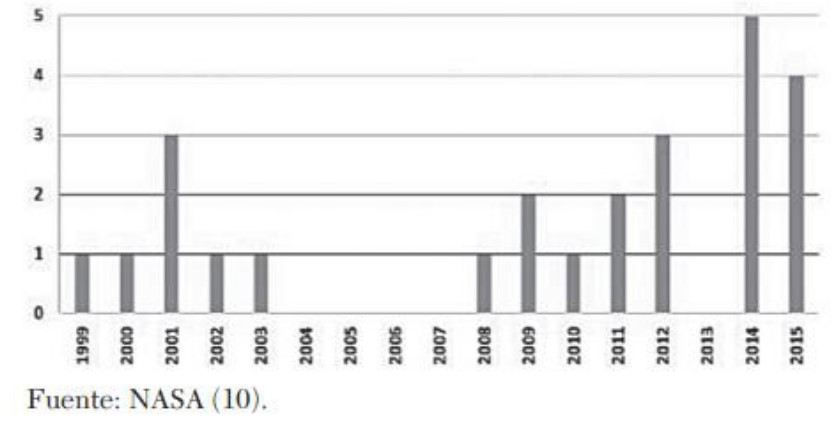
\includegraphics[scale=0.7]{Imagen/Imagen del articulo_page-0001.jpg}
\end{Figura}

\end{multicols}

\newpage 
%-----Pagina terminada----

%---------Pagina 12-------
\pagestyle{fancy}
        \fancyhf{}
        \rhead{}
        \lhead{\textsc{\tiny PERSONA Y BIOÉTICA • ENERO-JUNIO 201}}
        \lfoot{50}
        \cfoot{\scriptsize {ISSN 0123-3122 • e-ISSN 2027-5382 • pers.bioét. • Vol.22 • Núm. 1 • pp. 39-55 • 2018}}
\begin{multicols}{2}
\noindent Además del tiempo empleado para que una nave o
un satélite pueda ejecutar una maniobra evasiva, se
requiere también mucho dinero. Cuando un satélite
sale al espacio cuenta con un combustible limitado;
maniobrar para evadir una posible colisión consume
parte de ese combustible y reduce la vida útil de un satélite que puede costar cerca de 100 millones de euros.
Según la Comisión Europea, “solo las maniobras para
esquivar chatarra generan unos gastos de 140 millones
de euros al año y ese coste ascenderá a 210 millones
durante esta década debido al constante crecimiento
del basurero espacial” (25).
\section*{\noindent \small {AFECTACION DE LAS PERSONAS Y COMUNIDADES EN LA SUPERFICIE TERRESTRE}}
\\

\noindent Parece claro que la actual presencia de la basura espacialrepresenta un riesgo real para el éxito de las actuales y
futuras misiones espaciales, así como para el desempeño
ordinario de los satélites activos. Pero ¿existe un peligro
para los individuos o las poblaciones humanas sobre la
superficie terrestre? Según E. García Llama se calcula
que, solo en 2015, cerca de 450 residuos orbitales
(satélites, etapas y escombros) habrían reentrado a
la atmósfera terrestre. Como el 70\% de la superficie
terrestre está cubierta por agua, la mayoría de estos
objetos, cuando no se desintegran por la fricción con la
atmósfera, terminan en el mar. Además, solo un 1\% de
la superficie de la Tierra estaría poblada, lo que reduciría
aún más las probabilidades de que un cuerpo de este
tipo afecte la integridad física de los seres humanos.
\\

\noindent En noviembre de 2015, la página web del periódico El
mundo de España alertaba que en menos de 12 días se
habrían encontrado en Murcia tres objetos de basura
espacial. Se trataba de unas esferas metálicas recubiertas de carbono que probablemente servían como depósitos auxiliares  de  
\\
\\
\\
combustible.  Miguel  Belló,  director  de  la  empresa  privada Elecnor  Deimos,  responsable  del  observatorio  de  basura  espacial  de  Puertollano,  antes  mencionado, dio un parte de confianza al afirmar que la probabilidad de que un guante abandonado por un astronauta o cualquier fragmento proveniente del espacio caiga sobre nuestras cabezas es menor a la de que un rayo caiga sobre un ser humano (26). Pero, entonces, ¿no hay ningún peligro para la vida sobre la tierra?
\\

\noindent El mismo Belló afirma que un peligro real lo representan los satélites lanzados en las décadas de 1970 y 1980 que funcionaban con energía nuclear como uranio y plutonio. Ejemplo de ello es el satélite ruso Kosmos 954, lanzado por  la  URSS  en  1977.  Un  fallo  en  el  sistema  provocó  que el satélite reentrara al año siguiente en la atmósfera terrestre y, al caer, se esparcieran los residuos nucleares en  una  zona  del  norte  de  Canadá.  La  operación  que  buscaba  recuperar  el  material  radiactivo  y  limpiar  un  área  contaminada  de  124.000  km2  se  conoció  como  Operación Luz de la Mañana (Operation Morning Light). Se recuperaron doce fragmentos del satélite, la mayoría de  los  cuales  presentaba  radiactividad.  Canadá  pidió  a  la URSS más de 6.000 millones de dólares canadienses, correspondientes  a  los  gastos  de  recuperación  de  los  restos  del  satélite,  descontaminación  de  sus  territorios  y eventuales daños, de los cuales la URSS solo canceló una mínima parte (3 millones de dólares canadienses).
\\

\noindent Pero el Kosmos 954 no era el único satélite que funcionaba con energía nuclear en fallar. También lo hicieron los sa-télites rusos Kosmos 1402, el Kosmos 1900 y, por Estados Unidos, el SNAP-10 A. Se calcula que aún quedan cerca 40 de estos satélites “radiactivos” orbitando alrededor de la Tierra, cuya reentrada en la atmósfera y eventual caída sobre la superficie terrestre representan un peligro real.
\newpage 
%-----Pagina terminada----

%---------Pagina 13-------
\end{multicols}
\pagestyle{fancy}
        \fancyhf{}
        \rhead{}
        \lhead{\textsc{\tiny ASPECTOS BIOÉTICOS RELACIONADOS CON LA BASURA ESPACIAL Y SUS EFECTOS SOBRE LA VIDA...• l JUAN GUILLERMO DELGADO-MARTÍNEZ Y OTRO}}
        \rfoot{51}
        \cfoot{\scriptsize {ISSN 0123-3122 • e-ISSN 2027-5382 • pers.bioét. • Vol.22 • Núm. 1 • pp. 39-55 • 2018}}
\begin{multicols}{2}
\noindent Ciertamente, el peligro de la caída de basura espacial
en la superficie terrestre no se compara con la amenaza
que representa la caída de asteroides, ya que estos
últimos pueden presentar tamaños y velocidades mucho
mayores y, por tanto, su capacidad de destrucción es
bastante considerable. Existen unos 20.000 objetos
de más de 100 m cercanos a la Tierra, de los cuales se
habrían identificado menos de la mitad. Se piensa que el
famoso meteoro de Tunguska, que entró en la atmósfera
de Siberia el 30 de junio de 1908 y explotó en el cielo,
cerca del río Podkamenyana Tunguska, liberando una
energía similar a la de 185 bombas de Hiroshima (27),
tenía cerca de 37 m de diámetro. No es extraño, pues,
que el reconocimiento y seguimiento de asteroides que
pudieran cruzarse con la órbita de la Tierra no sea ya
solo un argumento de la ciencia ficción (28), sino objeto
de importantes proyectos espaciales (29).
\\

\noindent Quizá la mayor prueba de que la basura espacial es un
asunto para tener en cuenta sean las iniciativas de las
agencias espaciales de distintos países (que durante
décadas han lanzado y siguen lanzando satélites) para
mitigar el problema; estas parecen ser las más conscientes
de lo que está en juego. Entre las medidas que se
proponen están algunas recomendaciones internacionales
entre agencias para evitar la proliferación de basura
espacial, el estudio de las reentradas atmosféricas
para alertar sobre una eventual caída de restos sobre
poblaciones humanas, el esfuerzo por minimizar los
riesgos de explosiones en el espacio agotando la energía
y el combustible residuales al final de la vida útil de los
satélites, el diseño de nuevos satélites con materiales y
formas que reduzcan al mínimo la cantidad de residuos de
una eventual explosión o colisión, o incluso la planificación
y el diseño de satélites “recolectores de basura” que
serían capaces de interceptar la basura espacial para
lograr su reingreso a la Tierra.
\section*{ \small {SOLUCIONES BIOETICAS}}\\
\noindent ¿Qué puede decir la bioética frente al creciente
problema de la basura espacial? No cabe duda que, de
incrementarse, la presencia de residuos espaciales podría
poner en peligro la vida humana y animal de diversas
maneras, sea en el espacio, sea en la superficie terrestre. 
\subsection*{\normalsize{{\textit{Peligros para la vida en el espacio}}}}\\
\noindent La película de ciencia ficción Gravity (2013), del director mexicano Alfonso Cuarón, representa la destrucción de
la ISS y la muerte de casi toda su tripulación a causa
de múltiples colisiones causadas por los fragmentos
resultantes de una explosión previa. Aunque resulte
bastante improbable la destrucción de la ISS a causa de
una colisión de este tipo (30), no se pueden desestimar
los peligros de la basura espacial para la vida y salud de
los tripulantes de misiones espaciales. Las crecientes
maniobras evasivas o de inicio de evacuación por parte
de naves tripuladas, como la de la ISS, mostrarían que
la colisión con restos de basura espacial no sería solo
material de ciencia ficción. 
\subsection*{\normalsize{{\textit{Peligros para la vida en la tierra}}}}\\
\noindent Por otra parte, la vida sobre la superficie terrestre
podría verse afectada por una eventual caída de restos
de satélites, algunos de los cuales pueden contener
radiactividad, lo que afectaría amplias zonas habitadas
por seres humanos, especies animales o plantas. También
se ha mencionado una posible afectación, no solo para
la vida en el sentido biológico, sino entendida de forma
cultural, como modo de vida. Una buena parte de los
seres humanos depende de las tecnologías derivadas de
los satélites para efectos de comunicación, transporte
\end{multicols}
\newpage
%-----Pagina terminada----

%---------Pagina 14-------

\pagestyle{fancy}
        \fancyhf{}
        \rhead{}
        \lhead{\textsc{\tiny PERSONA Y BIOÉTICA • ENERO-JUNIO 201}}
        \lfoot{52}
        \cfoot{\scriptsize {ISSN 0123-3122 • e-ISSN 2027-5382 • pers.bioét. • Vol.22 • Núm. 1 • pp. 39-55 • 2018}}
\begin{multicols}{2}
\noindent (GPS), acceso a información, entretenimiento, fines
militares, así como el seguimiento y control de fenómenos
atmosféricos y naturales como incendios, huracanes,
entre otros, lo que tiene repercusiones no solo en el
plano cultural, sino vital. Conocer el origen, la evolución
y eventual dirección de un huracán o incendio puede ser
decisivo para brindar información oportuna, así como
para la toma de decisiones.
\\

\noindent La bioética, o mejor, los bioeticistas, pueden hacer un
aporte considerable al informar a la comunidad sobre
los riesgos de un incremento de la basura espacial, al
contribuir a generar consensos y políticas que busquen
reducir los lanzamientos o mitigar los impactos de la
basura espacial; al estudiar y alertar sobre los eventuales efectos de la caída de restos sobre las poblaciones
humanas y animales, en particular, si hubiese peligro de
caída de material radiactivo.
\\

\noindent Surgen aquí, además de las ya presentadas, muchas
preguntas éticas. ¿Se debería detener por completo el
lanzamiento de nuevos satélites y misiones espaciales
hasta tanto no se logre una reducción significativa de la
basura espacial en la órbita baja de la Tierra? ¿Es justo
que algunos países que apenas inician su “carrera espacial” se inhiban de lanzar satélites al espacio, mientras
que otros países pioneros de la exploración espacial
cuentan con cientos de satélites funcionales? ¿Estaría
obligada la agencia militar de Estados Unidos a revelar
información con el fin de evitar una eventual colisión con
basura espacial? ¿Es ético el uso de satélites espías por
parte de algunos países? ¿Debería haber una normativa
clara que regule y promueva eficazmente la reducción
de basura espacial? ¿Es posible lograr un consenso en
este punto cuando no existe una agencia que agrupe y
regule el actuar de todas las agencias espaciales? ¿Es ético usar energía nuclear en sondas y satélites que se envían al espacio? ¿Qué se debería hacer con los restos de  satélites  potencialmente  peligrosos,  por  contener  energía nuclear, que orbitan la Tierra?
\section*{ \small {CONCLUSIONES}}\\
\noindent En 1978, la bioética fue definida en la Enciclopedia de
Bioética como un “estudio sistemático de la conducta
humana en el área de las ciencias de la vida y de
la salud, examinado a la luz de los valores y de los
principios morales” (31). Como se ha visto, la bioética
contemporánea ha dado un giro al considerar no solo la
conducta humana en las específicas áreas de la vida y la
salud, sino que también intenta confrontar críticamente
los alcances y las implicaciones éticas sobre la vida en
general y de los desarrollos científicos y tecnológicos.
La conquista del espacio, y la proliferación de la basura
asociada a esta empresa, bien pueden entrar en el campo
de estudio de la bioética. Aunque la carrera espacial
y sus residuos difícilmente podrían ser considerados
como parte integrante de las ciencias de la vida y de
la salud, se ha intentado mostrar cómo pueden llegar
a afectar la salud y la vida, no solo de los tripulantes de
las misiones espaciales, sino de las poblaciones sobre la
superficie terrestre.
\\

\noindent Es una realidad que las diferentes etapas de la carrera
aeroespacial han presentado una carencia marcada de
los aspectos bioéticos,3si bien es cierto que en esas
etapas se ha considerado la seguridad de los animales
y de los seres humanos implicados, y, por supuesto, el
aseguramiento de las inversiones económicas.
\\

\noindent Es evidente que la preocupación propia de la bioética
por el futuro de la vida no pasa solo por los dilemas y 

\end{multicols}
\newpage
%-----Pagina terminada----

%---------Pagina 15-------

\pagestyle{fancy}
        \fancyhf{}
        \rhead{}
         \lhead{\textsc{\tiny ASPECTOS BIOÉTICOS RELACIONADOS CON LA BASURA ESPACIAL Y SUS EFECTOS SOBRE LA VIDA...• l JUAN GUILLERMO DELGADO-MARTÍNEZ Y OTRO}}
        \rfoot{53}
        \cfoot{\scriptsize {ISSN 0123-3122 • e-ISSN 2027-5382 • pers.bioét. • Vol.22 • Núm. 1 • pp. 39-55 • 2018}}
\begin{multicols}{2}
\noindent trilemas éticos del sector clínico. En ese sentido, la bioé-tica ha logrado entender que la misma vida humana que pretende cuidar y preservar se encuentra en relación con el equilibrio medioambiental y, por ello, prácticamente cualquier acción humana que suponga una intervención problemática con la vida entraría en su campo de estudio. En este frágil equilibrio que posibilite, por un lado, el éxito de la actividad científica y, por otro, la supervivencia de una vida siempre vulnerable frente a la acción humana, se encuentra también el espacio exterior.
\\

\noindent La existencia y las implicaciones de la basura espacial parecen un tema poco conocido para muchos, dado el carácter aparentemente “invisible” del acontecimiento, además del hecho de que afectaría principalmente los intereses económicos y políticos de algunos Estados o empresas  privadas,  y  no  a  los  ciudadanos  ordinarios.  Esto  no  es  del  todo  cierto  ya  que  grandes  sistemas  de  comunicación  y  meteorología  dependen  del  buen  funcionamiento  de  los  satélites  que  orbitan  la  Tierra,  y por tanto a esta “telépolis” (32) o tercer entornoque ha cambiado profundamente las formas de vida de las sociedades desarrolladas. Por otra parte, la basura espacial no solo afectaría el presente y futuro de la investigación espacial, sino que pone en peligro la seguridad de los astronautas en las misiones espaciales, así como la vida en  la  Tierra  por  cuenta  de  unas  cuantas  decenas  de  satélites que se enviaron el siglo pasado y que funcionan o funcionaron con energía nuclear que, de precipitarse a la Tierra, podrían ocasionar graves daños ecológicos en las zonas afectadas. De allí la necesidad de ponderar los valores y disvalores en juego (los riesgos), y considerar las  implicaciones  futuras  de  la  presencia  y  eventual  aumento de la basura espacial (33).
\\

\noindent Muchos  de  los  problemas  de  salud  que  afrontan  las  tripulaciones humanas (astronautas y cosmonautas) ya se conocen. El Programa de Investigación en Humanos de la NASA ha identificado 32 riesgos de salud relacionados con el espacio que se estudian en busca de nuevos enfoques de  prevención,  tratamiento  y  mitigación.  También  se  han  establecido  límites  aceptables  y  parámetros  de  exposición a estos riesgos. El marco ético propuesto por la Academia Nacional de Ciencias de Estados Unidos sobre la actividad de los astronautas recalca la importancia de  la  decisión  voluntaria  y  autónoma  de  cada  uno  de  ellos de participar en una misión, y de la garantía de la igualdad de oportunidades y de un proceso justo en la selección de tripulaciones (34).
\section*{ \small {AGRADECIMIENTOS}}\\
\noindent A  los  organizadores  del  Tercer  Congreso  Internacio-nal de  Astrobiología,  NASA-Astrobiology  Institute/Instituto  de  Astrobiología-Colombia,  que  se  celebró  en Manizales (Colombia), del 18 al 22 de octubre de 2016, que invitaron a realizar la ponencia y aprobaron la presentación en el evento; al Instituto de Astrobiología de Colombia por otorgar la beca de participación activa del primer autor, y a la Asociación Colombiana para el Avance de la Ciencia (ACAC) por la beca de participación activa al segundo autor.\\
\\
\textbf{Conflicto de intereses:} ninguno declarado.

\end{multicols}
\newpage
%-----Pagina terminada----

%---------Pagina 16-------

\pagestyle{fancy}
        \fancyhf{}
        \rhead{}
        \lhead{\textsc{\tiny PERSONA Y BIOÉTICA • ENERO-JUNIO 2018}}
        \lfoot{54}
        \cfoot{\scriptsize {ISSN 0123-3122 • e-ISSN 2027-5382 • pers.bioét. • Vol.22 • Núm. 1 • pp. 39-55 • 2018}}
\begin{multicols}{2}

\begin{center}
\begin{tabular}{c}\hline
    \noindent \small {\textcolor{white}{------------------------}REFERENCIA\textcolor{white}{------------------------}} \\\hline
\end{tabular}

\end{center}
\begin{enumerate}
    \item {\scriptsize López-Quintás A. La palabra manipulada. Madrid: Rialp; 2015.}
    
    \item {\scriptsize Postigo-Solana E.  Bioética  personalista:  ciencia  y  controver-sias. En: Tomás y Garrido G Postigo-Solana, E. Concepto de bioética  y  corrientes  actuales.  Madrid:  Ediciones  Internacio-nales Universitarias; 2007.}
    
    \item {\scriptsize Potter VR. Bioética puente, bioética global y bioética profun-da. Cuadernos del Programa Regional de Bioética OPS/OMS. 1998; 7. Disponible en: https://es.scribd.com/doc/215707369/Van-Rensselaer-Potter-Bioetica-puente-Bioetica-global-y-Bioetica-profunda}
    
    \item {\scriptsize Beauchamp  TL  Childress  JF.  Principios  de  ética  biomédica.  Barcelona: Masson; 1999.}
    
    \item {\scriptsize Organización  Mundial  de  la  Salud.  Reglamento  sanitario  in-ternacional. 2ª ed. Ginebra: OMS; 2005.}
    
    \item {\scriptsize Agencias DPA / EFE. Diario El Comercio. Se registra el ni-vel de contaminación más grave del año en Pekín. 4 de marzo (11:15). 2016. Disponible en: http://www.elcomercio.com/ten-dencias/nivel-contaminacion-pekin-china-alerta.html.}
    
    \item {\scriptsize Sarmiento-Medina  PJ.  Bioética  y  medio  ambiente:  introduc-ción  a  la  problemática  bioético-ambiental  y  sus  perspectivas.  Persona y Bioética. 2001;5(13-14):6-35.}
    
    \item {\scriptsize Cinemanet. WALL·E Batallón de limpieza [visitado 2017 abr 29]. 2008. Disponible en: https://www.cinemanet.info/2008/12/wall-e/}
    
    \item {\scriptsize De la Torre C. Acontecimientos y personajes históricos de la década  de  los  60.  La  carrera  espacial.  En:  La  EGB.  Recuer-dos de mi infancia en los años 60 y 70. [visitado 2016 oct 12]. Disponible  en:http://yofuiaegb.blogspot.com.co/2016/10/yo-fui-egb-recuerdos-de-los-anos-60-y-70-carrera-espacial.html}
    
    \item {\scriptsize García Llama E. El preocupante aumento de la basura especial. El Mundo. 2016. Disponible en: http://www.elmundo.es/blogs/elmundo/apuntesnasa
    /2016/05/17/el-preocupanteaumento-de-la-basura.htm}
    
    \item {\scriptsize Kessler   DJ.   Collisional   cascading:   The   limits   of   popula-tion  growth  in  low  earth  orbit.  Advances  in  Space  Re-search. 1991;11(12):63-66}
    
    \item {\scriptsize Wikipedia. Lista de todas las misiones espaciales lanzadas. 2016 [visitado 2017 abr 27].Disponible en: 
    https://es.wikipedia.org/wiki/anexo:misionespaciales}

    \item {\scriptsize García-Llama E. Sobre la basura espacial. 2016. Disponible en: http://www.investigacionyciencia.es/blogs/tecnologia/5
    /posts/sobre-la-basura-espacial-14225}
    
    \item {\scriptsize Echeverría-Ezponda FJ. Ciencia y valores. Barcelona: Edicio-nes Destino; 2002.}
    
    \item {\scriptsize Gutiérrez P. ¿Por qué la basura espacial podría dejarnos aisla-dos del espacio exterior? 2012. Fayer Wayer, Columna}
    
    \item {\scriptsize Navarro  C.  ¿Qué  es  la  basura  espacial?  ¿Cuál  es  su  origen?  ¿Por qué es importante deshacerse de la basura espacial? 2015. Disponible en: https://medium.com/@KisshanNavarro/basura-espacial-341e644b4c72#.c0oojo9dy)20}
   
    \item {\scriptsize Oliveira J. La órbita en la que se “entierran” los satélites artificia-les. 2017.  Disponible en:https://elpais.com/elpais/2017/07/11/cie
    ncia/1499764731_013050.html}
    
    \item {\scriptsize Kelso  TS.  Conceptos  básicos  de  la  órbita  geoestacionaria.  Satellite  Times.  1998  [visitado  2017  abr  29].  Disponible  en: http://celestrak.com/columns/v04n07/}
    
    \item {\scriptsize Krag H. The Inter-Agency Space Debris Coordination Com-mittee  (IADC).  An  overview  for  the  IADC  annual  activi-ties.  2017.  Disponible  en:  http://www.iadc-online.org/index.cgi?item=docs_pub}
    
    \item {\scriptsize Álvarez-León  R.  La  basura  aeroespacial,  otro  invento  del  hombre  que  también  nos  acorrala  día  a  día  y  afecta  nuestra  ecología humana. XX Congreso Internacional Ciencia y Vida. Universidad Libre Internacional de las Américas, ULIA / Uni-versidad Católica de La Plata (UCDLP). República Argentina. “La vida humana y la preservación de la casa común”. La Plata (Argentina), agosto 3-6 de 2016 [visitado 2017 abr 29]. Dispo-nible en: www.ucalp.edu.ar, www.ulia.org}
    \end{enumerate}
    \end{multicols}
    \newpage
%-----Pagina terminada----

%---------Pagina 17-------
    \pagestyle{fancy}
        \fancyhf{}
        \rhead{}
         \lhead{\textsc{\tiny ASPECTOS BIOÉTICOS RELACIONADOS CON LA BASURA ESPACIAL Y SUS EFECTOS SOBRE LA VIDA...• l JUAN GUILLERMO DELGADO-MARTÍNEZ Y OTRO}}
        \rfoot{55}
        \cfoot{\scriptsize {ISSN 0123-3122 • e-ISSN 2027-5382 • pers.bioét. • Vol.22 • Núm. 1 • pp. 39-55 • 2018}}
    
\begin{multicols}{2}
\begin{itemize}
    \item[21] {\scriptsize Courty JM, Kierlik E. Limpieza electromagnética del espacio. Como eliminar la chatarra espacial del entorno terrestre? IyC. 2015;465:86-87.}
    
    \item[22] {\scriptsize Rivera A. Un observatorio de basura espacial comienza a operar en Puerto Llano. 2016 [visitado 2017 abr 29]. Disponible en: https://el pais.com/elpais/2016/05/14/ciencia/1463243430_919708.html}
    
    \item[23]{\scriptsize Stansbery G. NASA´s Orbital Debris Program Office. Briefing to the NASA Advisory Council; 2016.}
    
    \item[24]{\scriptsize García Lama E. Sobre la basura espacial.IyC.2016.[visitado 2016 dic 8]. Disponible en: http://www.investigacionyciencia.
    es/blogs/tecnoloia/35/posts/sobre-la-basura-espacial-14225}
    
    \item[25]{\scriptsize Europa busca voluntarios para combatir la basura espacial. 2013 [visitado 2016 oct 12]. Disponible en: Disponible en: http://esmateria.com/2013/03/19/europa-busca-voluntarios-para-combatir-labasura-espacial/ 19 de septiembre de 2016.}
    
    \item[26]{\scriptsize Guerrero T. Los riesgos de la basura espacial. Diario El Mundo.2015 [visitado 2016 feb 14]. Disponible en:http://www.elmundo.es/ciencia/2015/11/17/564a31f0ca
    474187228b4640.html}
    
    \item[27]{\scriptsize NASA Beta. El evento de Tunguska - Cien años después. 2008 [visitado 2016 oct 12]. Disponible en: Disponible en:
    https://ciencia.nasa.gov/science-at-nasa/2008/30jun_tunguska/.}
    
    \item[28]{\scriptsize Killer Asteroids. Impact: Earth, what are the odds? 2010. [visitado 2017 may 17]. Disponible en: Disponible en: http://www.killerasteroids.org/.}
    
    \item[29]{\scriptsize Center for Near Earth Object. Top News Stories [visitado 2017 may 17]. Disponible en: Disponible en: http://neo.jpl.nasa.gov/.}
    
    \item[30] {\scriptsize Delgado-Martínez JG, Barriga LF. La vida es bella. Entrevista con Benjamín Virgil-Bastida [visitado 2017 mar 19]. Disponible en: Disponible en: http://lavidaesbellaradioucm.blogspot.com.co/2017/03/houston-hay-un-basurero-alla-afuera.html.}
    
    \item[31] {\scriptsize Reich W. Enciclopedia de Bioética, vol. 1. New York; 1978}
    
    \item[32] {\scriptsize Echeverría-Ezponda FJ. Telepolis. Barcelona: Ediciones Destino ; 1994}
    
    \item[33] {\scriptsize Echeverría-Ezponda FJ. Los riesgos de la globalización. En: Lujan-López JL, Echeverría-Ezponda FJ (eds.). Gobernar los riesgos. Ciencia y valores en la sociedad del riesgo. Madrid: OEI, Biblioteca Nueva; 2004.}
    
    \item[34] {\scriptsize Rivera A. Ética ante los riesgos que corre un astronauta. El País. 2014 [visitado 2016 oct 12]. Disponible en: Disponible en: 
    https://elpais.com/sociedad/2014/04/07/actualidad/1396
    897124_486543.html.}
    
   \end{itemize}
   \begin{center}
\begin{tabular}{c}\hline
    \noindent \small {\textcolor{white}{------------------------}FILMOGRAFÍA\textcolor{white}{------------------------}} \\\hline
\end{tabular}

\end{center}
  
    \begin{enumerate}
        \item {\scriptsize Cuaron A. Gravity [película]. Warner Bros. Pictures. Estados Unidos; 2013.}
        \item{\scriptsize Stanton, A. Wall-E. [película]. Walt Disney Pictures. Pixar Animation Studios. Estados Unidos; 2008.}
    \end{enumerate}
\end{multicols}

\end{document}